%\graphicspath{{figures/integration}}

\section{Single-cell integration via Matching}
SCIM performs multi-modal single-cell integration in two steps.
First, we construct an integrated latent space using an adversarial autoencoder framework \cite{makhzani2015} wherein representations are invariant to their corresponding technologies,
inspired by a model proposed previously \cite{yang2019a} and further extended in ~\cite{yang2019b}.
In the second step, we perform a strong pairwise alignment of datasets from each modality via a cell-to-cell matching strategy that efficiently extracts cross-technology cell matches from the latent space.
SCIM assumes a shared latent representation between technologies but, unlike other approaches, does not require one-to-one or overlapping correspondences between feature sets.
SCIM scales well in the number of cells in the input through the use of neural-nets, end-to-end training and an efficient bipartite matching algorithm.
Finally, this training scheme allows for the addition of an arbitrary number of technologies, which can be trained in parallel.

\begin{figure*}[ht]
    \centering
    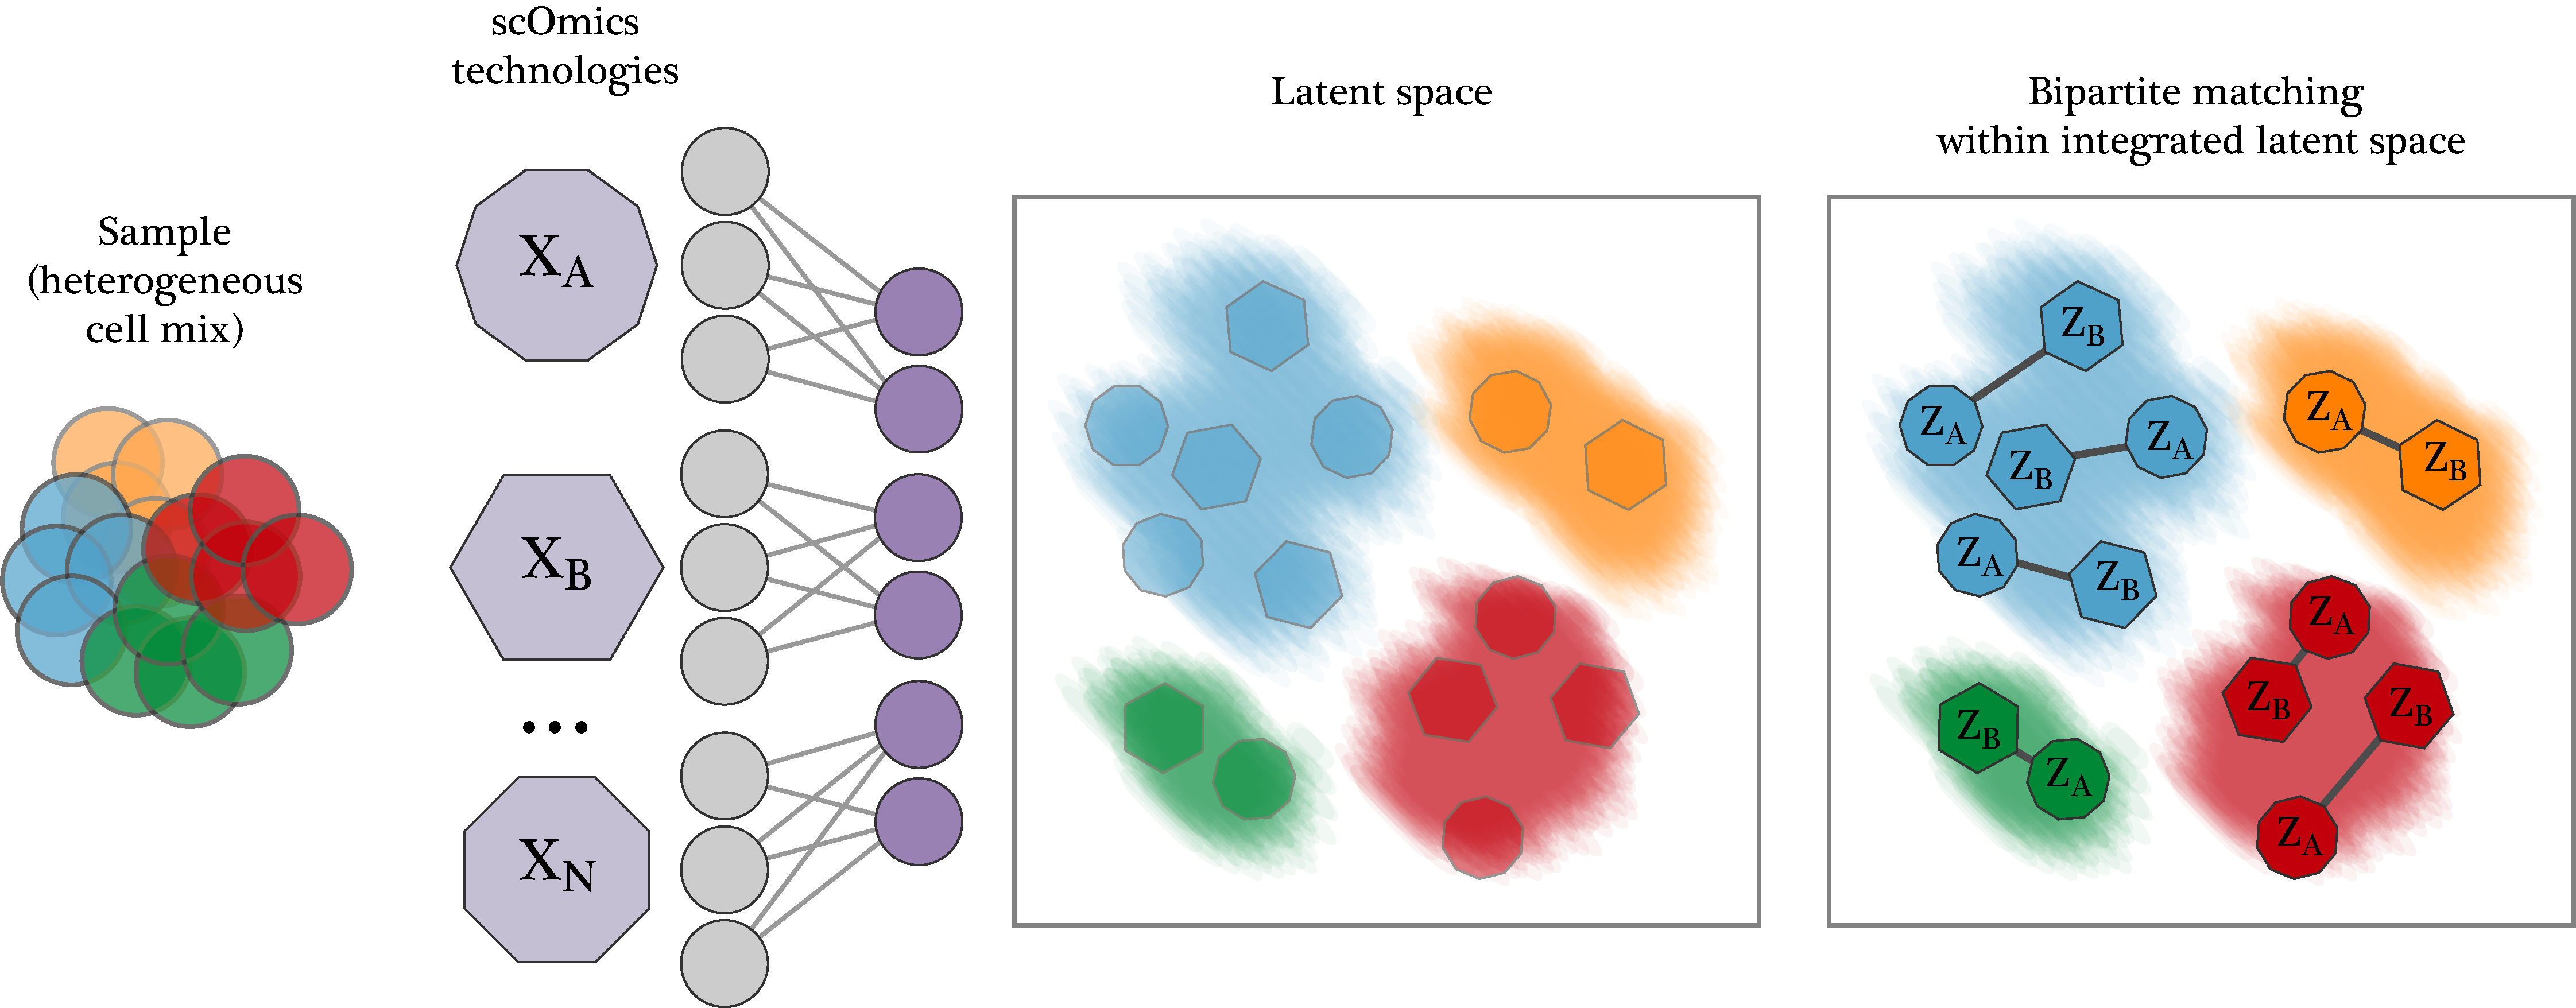
\includegraphics[width=\textwidth]{figures/integration/pipeline.png}
    \caption{
    SCIM performs a pairwise matching of cell across multiple single-cell 'omics technologies. We assume that the input of each technology comes from the same (or similar) heterogeneous cell mix, depicted on the left. Technologies generate a set of single cell 'omics datasets (violet polygons) in parallel (e.g. $X_A$, $X_B$, $X_N$).
    These datasets are represented as matrices of cells-by-features, where features are specific to the profiling technology, but could be gene expression, protein levels, etc.
    SCIM proceeds to map cells into a technology-invariant latent space (left box) using an autoencoder framework and an adversarial term to keep technologies well integrated.
    Here the latent representations capture the underlying structure in the cell mix (colored clouds) and analogous cells from different technologies (colored polygons) are placed in proximity.
    To integrate datasets, a fast bipartite matching scheme is applied, matching cells pairwise among datasets to cross-technology analogs, using their latent representations (right box).
    }
\end{figure*}

\subsection{Constructing technology-invariant representations}
SCIM encodes datasets into a shared latent space that is constructed to have two properties:
1) the inputs should be able to be reconstructed from their latent representations, as is typically achieved by vanilla VAEs
and 2) the latent representations of each technology should be well-integrated such that they are indistinguishable from each other.
In a successful integration the resulting latent space will have corresponding cells across all technologies represented in close proximity.

To construct an integrated latent space, SCIM uses a modified adversarial auto encoder framework.
This consists of the following networks: a pair of encoder ($\phi_k$) and decoder ($\psi_k$) networks for each technology $k$ and a single discriminator network ($\gamma$) acting on the latent space.
This discriminator is a binary classifier trained to identify the latent representation of some source technology from latent representations of all other technologies using a binary cross entropy loss.

SCIM yields an integrated latent space by minimizing the reconstruction error while adversarially fooling the discriminator.
Let $\mu$ and $\nu$ be the distribution of cellular states in the source $s$ and target modality $t$.
%Given the measurements of a batch of cells from the target modality $t$, $x_t$, and the (fixed) latent representations of a batch of cells from the source modality $s$, $\hat{z}_s \sim \phi_s(x_s)$,

\begin{equation}
	\min_{\phi_t, \psi_t} \max_\gamma  \
	\mathbb{E}_{x_t \sim \nu} \
	[ \mathcal{L}_{nll}(x_t, \phi_t, \psi_t) - \beta \mathcal{L}_{adv}(x_t, \phi_t, \gamma) ]
  \label{eq:scim-loss}
\end{equation}

$\mathcal{L}_{nll}$ is the negative log-likelihood of the inputs under their reconstruction.
$\mathcal{L}_{adv}$ is the error of the discriminator $\gamma$ to classify the latent representation of source samples $z_s = \phi_s(x_s)$ from target samples $z_t = \phi_t(x_t)$.
$\beta$ is a hyperparameter weighing the influence of the adversarial loss.

\paragraph{Latent space orientation}
Correctly orienting the latent space in an unsupervised manner is a challenging task \cite{locatello2019a, yang2019a}.
Consider, for example, a simple monotonic temporal process.
The latent representations for one dataset could be oriented from start to end, while another could be oriented from finish to start \cite{welch2017}.
Equation \ref{eq:scim-loss} satisfied, the representations are well integrated and inputs can be correctly reconstructed from them, yet the inter-dataset relationships are misaligned.
\citet{makhzani2015} address a similar problem by concatenating one-hot representations of labels reflecting intra-technology structure (e.g. cell type is an appropriate choice for ’omics datasets) to the discriminator inputs, showing that this supervision is necessary to orient the latent space.
Furthermore, \citet{locatello2019} argued that only a small number of labels are actually needed to achieve orientation.
To this end, we adopt a semi-supervised approach for some experiments by adding a ‘censored’ label and randomly relabel cells in the training set.

\paragraph{Model architecture}
Unless specified otherwise, we adopt the following architecture settings.
All networks use the ReLU activation \cite{agarap2019}.
We set the latent dimension of all models to eight, but observed this choice to be flexible.
We use discriminator networks with two layers and eight hidden units each.
The Spectral Normalization framework \cite{miyato2018} is used during training, which has been argued to stabilize discriminator training by effectively bounding its gradients.
We use a Gaussian activation for all decoders, a 2 layer architecture with 64 hidden units for all simulated data networks, a 2 layer architecture with 8 hidden units for all CyTOF networks and a 2 layer architecture with 64 hidden units for all scRNA networks.
The number of features and complexity of data is considered when choosing capacity and depth.

\paragraph{Optimization}
Optimization proceeds by iteratively fixing one technology as the source and one technology as the target.
In the case of more than two technologies, the technology corresponding to the discriminator’s positive class must either be the source or target technology.
Optimization proceeds with an inner and outer loop.
In a single inner loop step, the latent representations of the source technology are fixed and Equation \ref{eq:scim-loss} minimized with gradient updates to the encoder and decoder of the target modality $t$ using gradients computed on the batch $x_t$.
This process is repeated multiple times and then one step of the outer loop is performed.
In a single outer loop step, the discriminator is updated to classify $z_s$ and $z_t$.
All networks are optimized using the ADAM algorithm \cite{kingma2013}.


\paragraph{Model Selection}
Due to the min–max nature of adversarial training, model comparison is challenging since one cannot directly compare the minimized objective functions of converged models \cite{lucic2017}.
While the computer vision community has introduced a number of metrics specific to the image domain to help compare models \cite{heusel2017,salimans2016}, here we need to validate the quality of a set of lower-dimensional latent representations.
To achieve this, we utilize a k-Nearest Neighbor (kNN)-based divergence estimator \cite{wang2009}.
The divergence score between two sets of codes $Z_s$ and $Z_t$ is calculated as:
\begin{equation}
	\hat{D}(Z_s || Z_t) = \frac{1}{2} \hat{D}_{KL}(Z_s || Z_t) + \frac{1}{2} \hat{D}_{KL}(Z_t || Z_s)
\end{equation}
where $\hat{D}_{KL}$ is the KL divergence estimated from samples.
This estimator approximates a symmetric variant of a KL divergence, a measure of how much two distributions differ, using only empirical data.
The divergence estimate is computed between the latent representations of the source technology and the target technology to measure the alignment of codes from the two technologies.
Model selection can proceed at scale by selecting parameter configurations that align technology distributions and have low reconstruction error.

\subsection{Bipartite matching of single-cell embeddings}
In its second step, SCIM performs multi-modal integration by identifying pairs of corresponding cells across two modalities using their representations in the latent space constructed in the first step.
We identify pairs by solving a combinatorial bipartite matching problem \cite{ahuja1993,dellamico2000}, wherein the bipartite graph is constructed by connecting cells between each pair of technologies, weighted by their distances in the latent space.
The bipartite matching problem then identifies an optimal set of paired cells that minimizes the total edge cost of all matches.
In order to achieve this efficiently and at scale, we approximate the full bipartite graph with a k-Nearest Neighbors (kNN) graph that identifies a set of potential matches for each cell and reduces the complexity of the problem.
We then extend the graph to account for single-cell data characteristics and solve the bipartite matching within a general framework of Minimum-Cost Maximum-Flow problems \cite{ahuja1993,klein1967}.

\paragraph{Min\-cost Max\-flow matching}
Based on a Euclidean cost matrix, we aim at finding the maximum number of cell pairs with minimum cost.
This corresponds to finding a maximum flow that can be pushed through the graph, where each edge between cells has capacity 1, while minimizing the overall cost.
To solve the Minimum-Cost Maximum-Flow problem in a computationally efficient way we use an implementation of the network simplex algorithm \cite{kiraly2012}.

\paragraph{Evaluation}
Since it is not possible to profile the same cell in multiple modalities, we lack a set of ground truth cell pairs to evaluate against.
The integration quality is instead evaluated on several levels, specific to the samples and modalities integrated.
First, when cell type labels are present, the accuracy corresponding to the fraction of true positives with regard to cell-type label is reported.
Cell types can be determined in a technology-specific manner and the accuracy is reported on a common denominator.
If more fine-grained cellular information is available, such as pseudotime, a direct comparison of this quantity is carried out.
Furthermore, in real-world data settings we utilize the raw marker expression to investigate correspondence of the matched cells.
Namely, Spearman’s and Pearson’s correlation coefficients are computed between the expression values across matches.

%\subsubsection{Graph modifications}

\paragraph{kNN subgraph approximation}
Given the large number of cells in single-cell datasets, we reduce the search space to the $k$ most likely potential matches.
For each pairwise integration task, two kNN graphs are built: the first uses the source data queried by the target technology cells, and the second uses target data queried by the source technology
That is, each cell in the source technology is connected to its $k$ nearest neighbor cells in the target technology and each cell in the target technology is connected to its $k$ nearest neighbor cells in the source technology.
The union of this graph is then used in the bipartite matching solver.
The sparsity of these connections, regulated by the choice of the hyperparameter $k$, corresponds to a trade-off between the computational performance (memory usage, run time) and the final matching accuracy.

\paragraph{Null Cell}
The bipartite matching, Figure \ref{fig:null-cell} makes the assumption that each cell has a singular corresponding sibling in its paired technology.
However, it is reasonable to expect that differences between profiled samples exist that would invalidate this assumption.
To allow for mismatches due to this expected variation in cellular composition,
we expand the kNN graph with sparse connections by adding a densely connected \textit{null cell} with high capacity and relatively large edge weight. 
This allows to capture potentially poorly matched cells by keeping them unassigned.
The magnitude of the null match penalty is a hyperparameter that corresponds to a given percentile $p$ of the overall costs.

\begin{figure}
  \begin{center}
    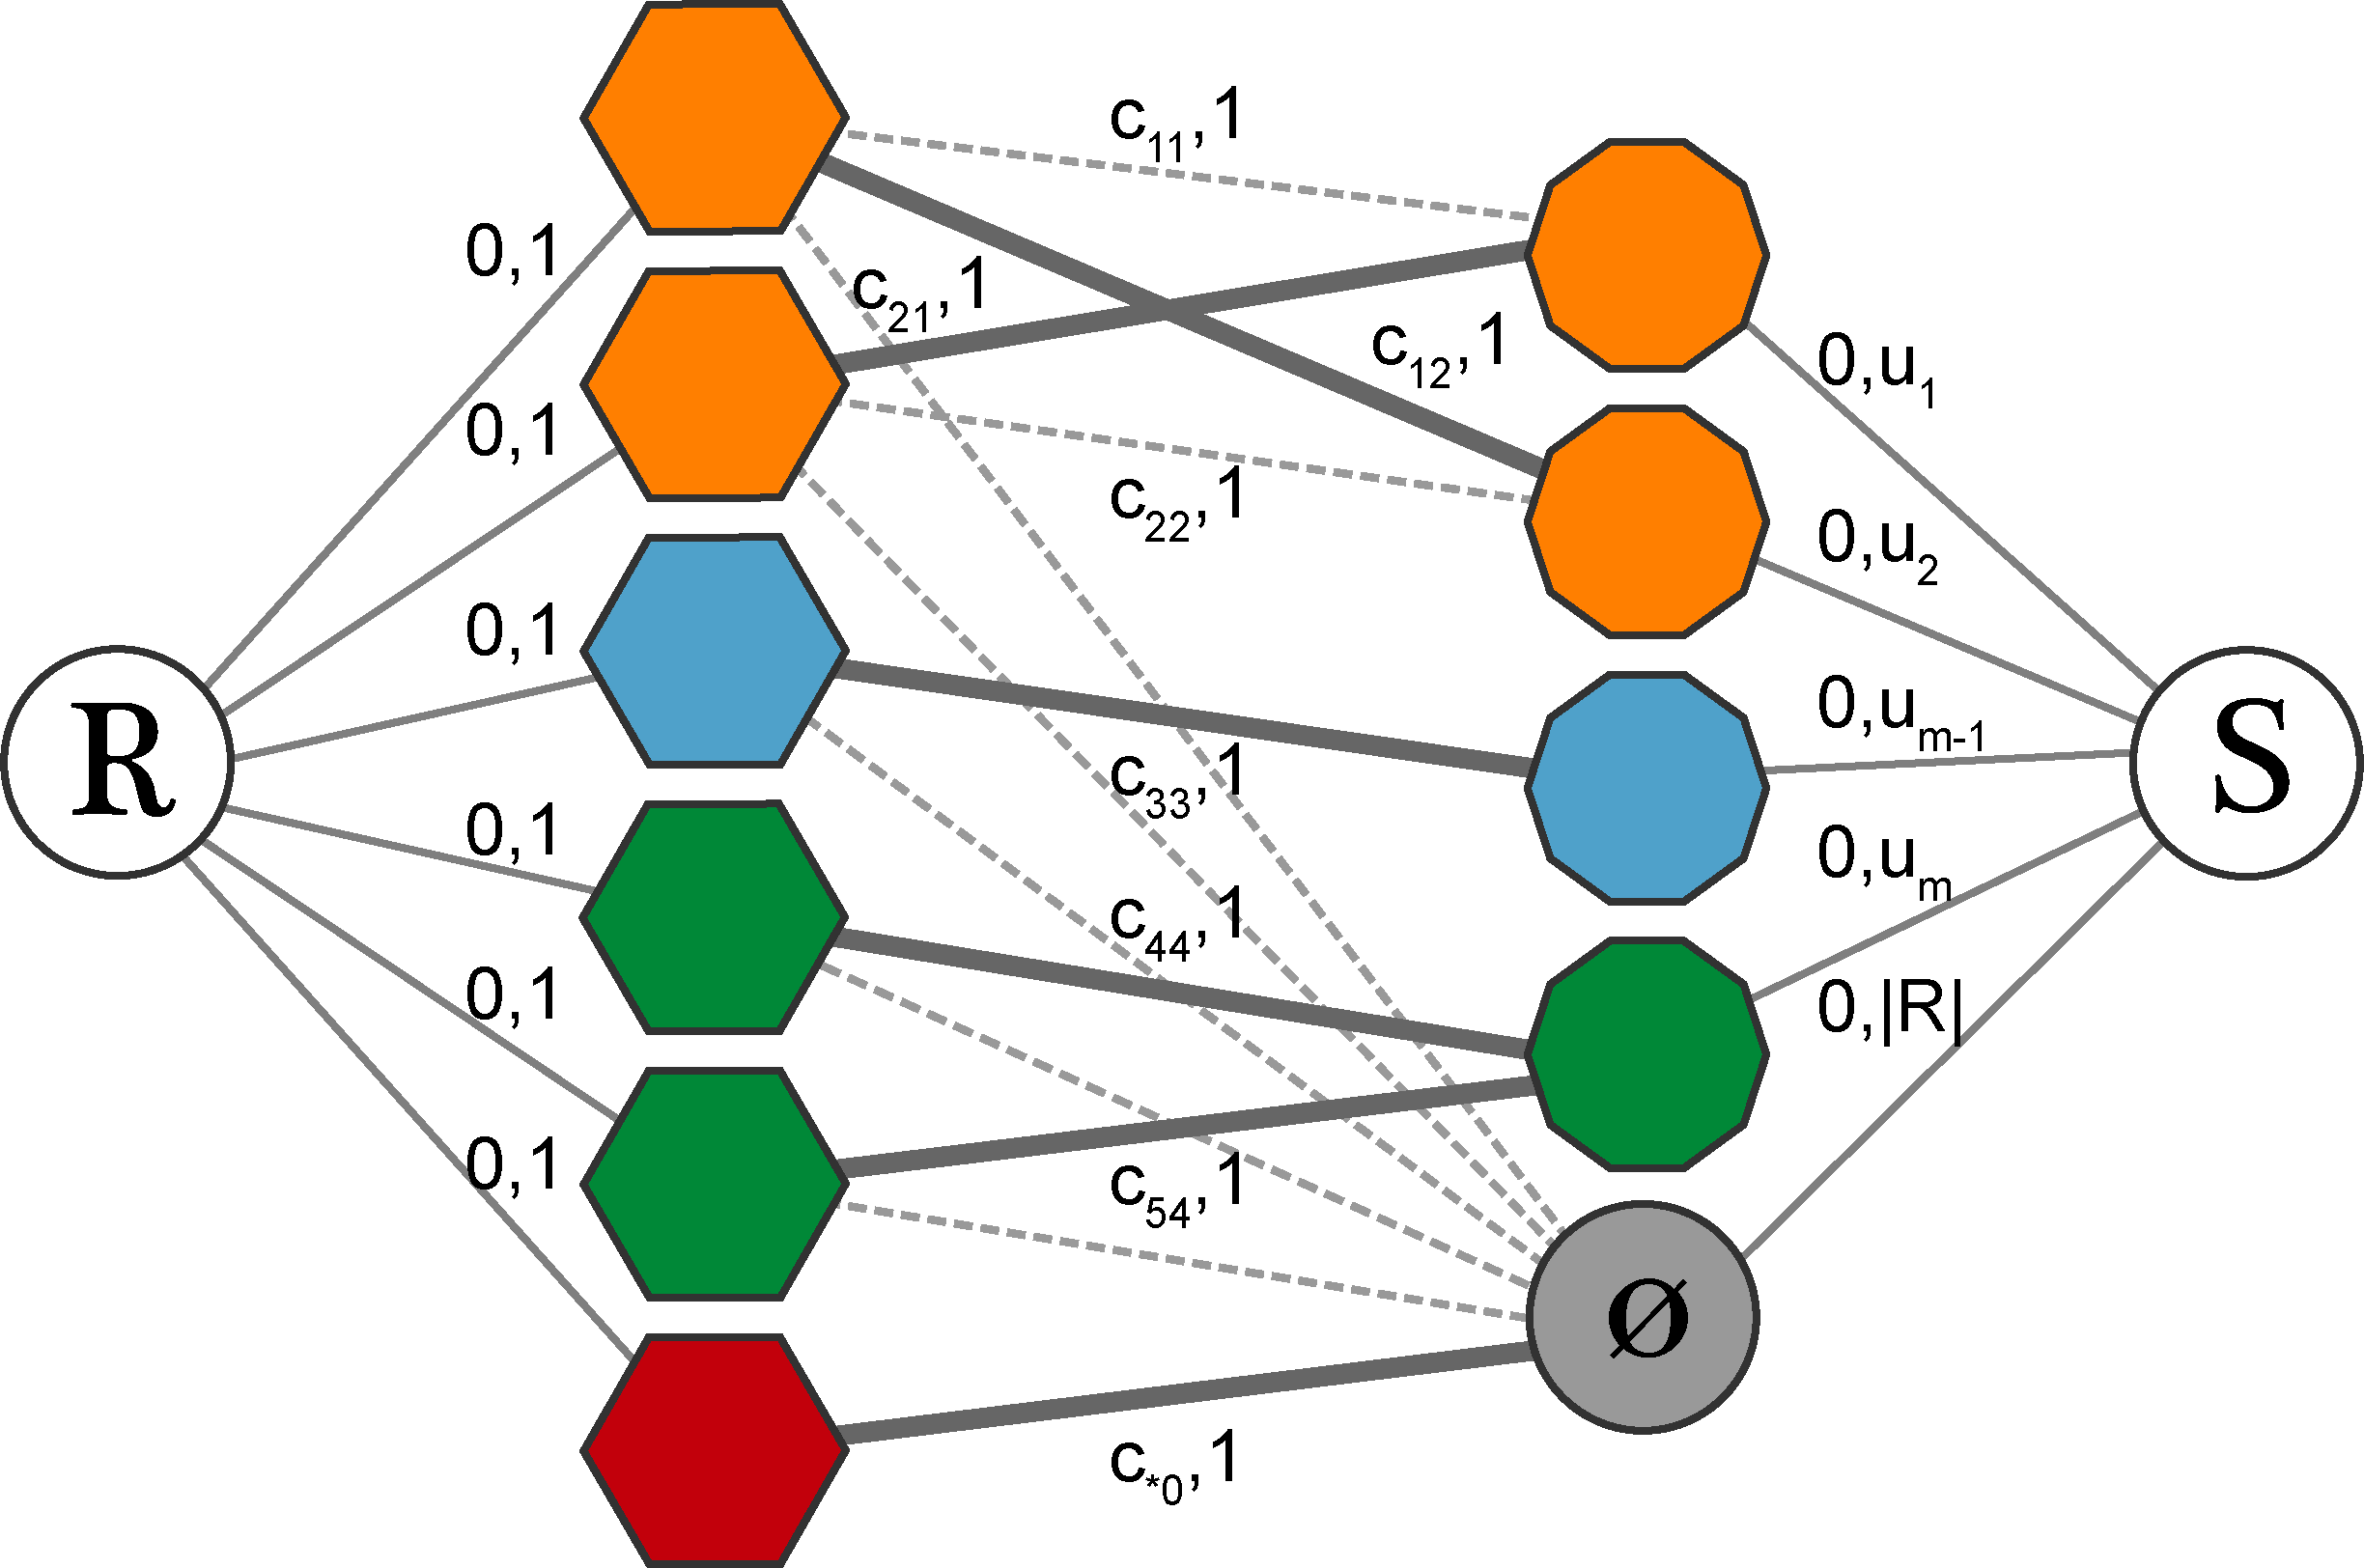
\includegraphics[width=0.95\textwidth]{figures/integration/null-cell.png}
  \end{center}
  \caption{Fast bipartite matching using a customized Minimum-Cost Maximum-Flow framework. Nodes correspond to cells with technology represented by shape, i.e. hexagons and decagons. R and S represent root and sink nodes. Edges correspond to the sparse connections between the cells, resulting from a kNN search. Edge labels indicate matching cost (first value) and edge capacity (second value). Many-to-one matches in unbalanced datasets are enabled by increasing the capacities ui (for i $\in$ 1;  . . ; m). The null node, colored in gray, captures matches of cells (from the bigger dataset on the left-hand side of the graph) that lack a close enough analog in the other technology. Its capacity equals the cardinality of the bigger dataset and the null match penalty is relatively high. The thicker lines linking the nodes represent the actual matches selected by the algorithm.}
  \label{fig:null-cell}
\end{figure}

The extended graph structure is depicted in Figure \ref{fig:null-cell}, where $R$ and $S$ refer to the root and sink nodes, respectively.
Furthermore, to account for differences in the number of cells between modalities ($n$, $m$), we allow for one-to-many matches by increasing the capacity of the edges incoming to the sink ($u_i$ for $i \in {1, \ldots, m}$, assuming the nodes linked to the sink correspond to the smaller dataset, i.e. $m \leq n$.
To prevent all matches from collapsing onto a very small set of nodes, we constrain the incoming sink capacities, excluding the null node, to equal the cardinality of the bigger dataset divided by the cardinality of the smaller dataset, with the capacities distributed uniformly across the sink edges.
If more than two data modalities are present, the bipartite matching is solved sequentially by obtaining pairwise matches between technologies.
